\chapter{Considerazioni Etiche e Legali}\label{chapter:Considerazioni}

Considerato quanto trattato finora, riconosceremo che navigare nel dark web con gli strumenti presentati, non è illegale di per sé, ma dipende sempre dalle azioni che si compiono e dalle ricerche che si effettuano.

Sarà legale accedere al proprio account di posta elettronica o al proprio profilo social. Sarà invece illegale accedere a una rete aziendale o governativa senza autorizzazione o a una banca dati protetta da copyright.

Il pericolo proverrà sempre dal contatto che si andrà ad avere con il dark web, dove materiali illegali e immorali sono all'ordine del giorno.

Esistono infatti diverse leggi e norme che regolano l’uso di internet e che vietano, e sanzionano, determinate attività o contenuti, mirando a garantire la protezione dei dati personali, il contrasto al cybercrime, la protezione della proprietà intellettuale e la prevenzione della diffusione di contenuti illeciti (come pornografia infantile, incitamento all'odio, terrorismo, e traffico di droga).

\'E fondamentale che le organizzazioni forniscano formazione continua in materia legale ed etica ai team che operano con l'OSINT e il dark web, implementino politiche interne allo scopo di definire chiaramente i limiti legali ed etici per l'utilizzo dell'intelligence. Queste policy devono riguardare l'uso di tutti gli strumenti dai software, ai dati, fino alle fonti di informazioni. 

\newpage
\section{Normative sulla Privacy}\label{sec:cap_sec_cons1}

Vediamo di seguito alcuni dei principali regolamenti di sicurezza (come GDPR, CCPA, PCI-DSS) utili a condurre audit\footnote{è una valutazione indipendente volta a ottenere prove, relativamente a un determinato oggetto e giudicarle con obiettività, per stabilire in quale misura i criteri prefissati siano stati soddisfatti o meno} per operare in conformità e in modo legale.

In particolare ne possiamo ritrovare di due tipologie, con una giurisdizione locale o nazionale.
Con giurisdizione locale avremo:\\

\textbf{Decreto Legislativo 70/2003 - Italia}
Questo decreto recepisce la Direttiva 2000/31/CE dell'UE, stabilendo disposizioni riguardanti il commercio elettronico, la responsabilità degli intermediari, e la tutela dei minori su internet.
Viene impiegato contro fornitori di servizi, anche sul dark web, che non adempiono agli obblighi di segnalazione dei contenuti illegali o che facilitano la diffusione di contenuti illeciti.\\

\textbf{Computer Fraud and Abuse Act (CFAA) - Stati Uniti}
\'E una legge federale degli Stati Uniti che disciplina l'accesso non autorizzato a computer e sistemi informatici in generale. Risulta in vigore dal 1986, è una legge utilizzata per perseguire reati di hacking, frodi informatiche, e attività di cracking.
La si utilizza per giudicare e perseguire chiunque e su qualsiasi livello del web (visibile o dark), acceda senza autorizzazione a un sistema informatico protetto.\\

\textbf{Digital Economy Act - Regno Unito}
Questo regolamento del 2017 include misure per il controllo dei contenuti online, come la pornografia e materiale di tipo estremista o terroristico, si concentra anche sul rafforzamento delle leggi contro la pirateria digitale.
Ne è soggetto chiunque operi nel web, compreso il dark web, e renda disponibili contenuti che infrangono il Digital Economy Act, l'offensore potrà essere soggetto a multe e ad altre sanzioni legali.\\

\textbf{Cybersecurity Law - Cina}
La legge sulla sicurezza informatica cinese impone controlli rigorosi sull'accesso a Internet e sull'utilizzo di dati all'interno del paese. \'E stata sviluppata per proteggere la sovranità digitale del paese, garantire la sicurezza nazionale e mantenere la stabilità sociale.
Ne è soggetta qualsiasi attività online, sia sul web visibile che nel deep o dark web, e prevede controlli rigorosi da parte delle autorità cinesi, comprese le attività che potrebbero essere considerate sovversive o dannose per l'ordine pubblico.\\

\'E poi importante sottolineare come diversi paesi ad oggi abbiano adottato leggi che vietano il traffico di stupefacenti, la vendita di armi, la tratta di esseri umani, il terrorismo e la diffusione di materiali illeciti.
In aggiunta a questo sono state predisposte una serie di autorità, come l'FBI negli Stati Uniti, l'Europol nell'UE (Unione Europea), insieme ad altre agenzie di polizia, per collaborare e monitorare il web ed in particolare il dark web e intraprendere azioni contro tali attività 

\begin{figure}[ht]
	\centering
	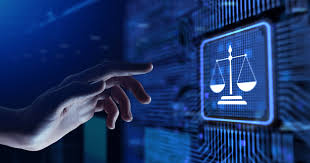
\includegraphics[width=0.8\textwidth]{Immagini/cons1.jpeg}
	\caption{La legge e la cybersecurity}
	\label{fig:onecons}
\end{figure}

\subsection{Regolamentazioni Internazionali}\label{subsec:es_subsec_cons1}

La Convenzione di Budapest è il quadro legale internazionale per affrontare i crimini informatici a livello globale, con un impatto esteso in tutto il mondo grazie all'adesione di molte nazioni. Il GDPR come la convenzione di Budapest ha un impatto globale grazie alla sua applicabilità extraterritoriale, influenzando la conformità alla protezione dei dati a tutte le aziende che trattano dati di cittadini dell'UE.\\

\textbf{La Convenzione di Budapest (Convention on Cybercrime) - Consiglio d'Europa}
La Convenzione di Budapest, aperta alla firma il 23 novembre 2001 a Budapest, Ungheria, ed entrata in vigore il 1º luglio 2004, è il primo trattato internazionale che mira a combattere il crimine informatico, è stata firmata da numerosi paesi in tutto il mondo, la maggior parte dei membri del Consiglio d'Europa, gli Stati Uniti, il Canada, il Giappone e molti altri.
Stabilisce norme minime per la legislazione nazionale relativa ai crimini informatici e promuove la cooperazione internazionale per indagini e azioni legali contro il cybercrime. Copre una vasta gamma di reati informatici, tra cui l'accesso non autorizzato, l'intercettazione illecita, la manipolazione di dati, e la pornografia infantile.\\

\textbf{Regolamento Generale sulla Protezione dei Dati (GDPR) - Unione Europea}
Anche se è principalmente una normativa dell'Unione Europea, il GDPR\footnote{Il GDPR è stato adottato il 27 aprile 2016, ed è entrato in vigore il 25 maggio 2018} ha un impatto internazionale. È applicabile a tutte le aziende, organizzazioni e entità, indipendentemente dalla loro ubicazione geografica, se trattano i dati personali di cittadini o residenti dell'UE.
Impone severi requisiti per la protezione dei dati personali e per la privacy, influenzando globalmente il modo in cui le organizzazioni trattano i dati degli utenti. La sua applicabilità extraterritoriale ha portato molte aziende al di fuori dell'UE ad adattare le loro pratiche per essere conformi alla normativa.\\

\textbf{Altri Accordi Internazionali di Cooperazione nel Contrastare il Cybercrime}
Oltre alla Convenzione di Budapest, ci sono altri accordi e protocolli internazionali che promuovono la cooperazione tra paesi per combattere il cybercrime. Questi possono includere accordi bilaterali o multilaterali tra paesi, per facilitare la condivisione di informazioni, l'estradizione di cybercriminali, e altre misure di sicurezza cibernetica.
Questi accordi sono solitamente basati sul diritto internazionale e promuovono una risposta coordinata alle minacce informatiche, considerando che il cybercrime spesso coinvolge più giurisdizioni.


\section{Limiti Legali e Implicazioni Etiche}\label{sec:cap_sec_cons2}

Sebbene l'OSINT utilizzi dati cosiddetti "aperti" o disponibili pubblicamente, c'è un dibattito etico su quanto sia giusto raccogliere informazioni personali (tecnicamente disponibili) senza il consenso dell'individuo. 
In quanto l'aggregazione massiccia di dati, la creazione di profili, o il tracciamento di comportamenti possono essere percepiti come una violazione della privacy.

Le profilazioni automatizzate attraverso strumenti OSINT possono introdurre bias (pregiudizio o allerta), con implicazioni negative per la privacy e la sicurezza individuale. Ad esempio, una persona può essere etichettata erroneamente come una minaccia o un sospettato basato su dati incompleti o errati.
Gli strumenti di monitoraggio del dark web e dell'OSINT, sbiadiscono la sottile linea tra la protezione proattiva e la sorveglianza ingiustificata, in quanto possono essere usati sia per scopi legittimi (come la sicurezza e la protezione della privacy) sia per scopi malevoli (come lo stalking o la manipolazione dei dati). 

Le organizzazioni che utilizzano tecniche OSINT e monitoraggio del dark web devono poi operare con trasparenza, informando le persone i cui dati potrebbero essere raccolti e analizzati. E in casi particolari ottenere il consenso per la gestione delle informazioni.
Gli analisti di cybersecurity e le aziende devono invece rispettare le best practices etiche e normative quando monitorano dati pubblici e il dark web. Ad esempio, quando si conducono ricerche su hacker particolarmente pericolosi, è necessario considerare i rischi di escalation o di danni collaterali.
